% =========================================================================
% Appendix K — pull-request roll. FILLED.
%   folds companion/pr-roll.json: the landed UFO PRs (spec #187, verify
%   V1-V4 #201/#216/#212/#206, CERN sibling #220), grouped by phase, the
%   monograph PR itself, roll totals, the schema, and a pgfplots PR-by-phase
%   chart. Honest: implementation mass is in hexa-lang (@D d3); UFO side is
%   pointer/manifest + absorption metadata.
% =========================================================================
\section{Pull-Request Roll}
\label{app:prroll}

This appendix is the transcription of the
\texttt{companion/pr-roll.json} session pull-request roll: every merged
PR that produced the UFO capstone, with its \texttt{gh}-measured
diff-stat. The records carry no synthetic data ---
\texttt{merged\_at}, \texttt{files\_changed}, and the line counts are
read back from \texttt{gh pr view --json}. The roll is grouped by phase:
Phase A (the 7-stage ladder folds), Phase B (the five sub-axes), Phase C
(the seven-verb pipeline, headed by the \texttt{spec} PR), Phase D (the
meta layer: LATTICE\_POLICY, LIMIT\_BREAKTHROUGH, CROSS-DOMAIN-MEGA,
EXPERIMENTS$+$HYPOTHESES), and the verify ladder (V1--V4), plus this
monograph PR itself. The implementation mass lives in hexa-lang (the
canonical code home, @D~d3); the UFO side is pointer/manifest and
absorption metadata only.

% -------------------------------------------------------------------------
\subsection{The landed-PR table}
\label{app:prroll-table}

Table~\ref{tab:prroll} is the roll transcribed from
\texttt{companion/pr-roll.json}. Where a line count reads ``---'' the
\texttt{gh}-measured value was not persisted in the companion record; we
do not invent one (@D~g3).

\begin{table}[h]
\centering
\footnotesize
\setlength{\tabcolsep}{4pt}
\begin{tabular}{@{}c >{\raggedright\arraybackslash}m{6.6cm} c c c@{}}
\toprule
\textbf{\#} & \textbf{title / role} & \textbf{merged} & \textbf{files} & \textbf{phase} \\
\midrule
187 & verb-1 \texttt{spec} --- single-pilot vehicle spec (7-stage matrix, LSS 12\,h, record-consume contract) & 2026-05-25 & 2 & C \\
201 & V1 claim inventory + tier triage (38-claim, \tierGreen9/\tierYellow8/\tierOrange4/\tierWhite17) & 2026-05-25 & 1 & verify \\
216 & V2 formal --- $n{=}6$ lattice integer identities (\tierBlue; atlas idempotent, fold 0) & 2026-05-25 & 1 & verify \\
212 & V3 numerical recompute --- Stage-1--3 nine \tierGreen\ verbatim ($|\Delta|\le10^{-9}$) & 2026-05-25 & 1 & verify \\
206 & verb-6 \texttt{verify} --- integrated digital-twin ledger (4-layer $\times$ tier matrix) & 2026-05-25 & 2 & C \\
220 & CERN sibling monograph (SCAFFOLD+BODY) --- the reference pattern this capstone mirrors & 2026-05-26 & --- & sibling \\
--- & \textbf{THIS PR} --- \texttt{ufo-capstone} monograph (scaffold + body + appendix A--L + companion + cover; \texttt{absorbed=false}) & --- & --- & monograph \\
\bottomrule
\end{tabular}
\caption{The UFO capstone pull-request roll
(\texttt{companion/pr-roll.json}). Schema per row:
\{\texttt{repo}, \texttt{number}, \texttt{title}, \texttt{merged\_at},
\texttt{files\_changed}, \texttt{lines\_added}, \texttt{lines\_deleted},
\texttt{phase}, \texttt{role}\}. The verify-ladder PRs (V1--V4, \#201,
\#216, \#212, \#206) and the verb-1 \texttt{spec} PR (\#187) are the
landed UFO-side records; \#220 is the CERN sibling whose structure this
monograph mirrors; the final row is the monograph PR itself.}
\label{tab:prroll}
\end{table}

% -------------------------------------------------------------------------
\subsection{Roll by phase}
\label{app:prroll-phase}

Fig.~\ref{fig:prroll} groups the roll by phase. The verify ladder
(V1--V4) is the densest, reflecting the capstone's verify-native
discipline; the pipeline (Phase C) carries the \texttt{spec} and
\texttt{verify} verbs; the sibling and monograph rows are the reference
pattern and this volume.

\begin{figure}[h]
\centering
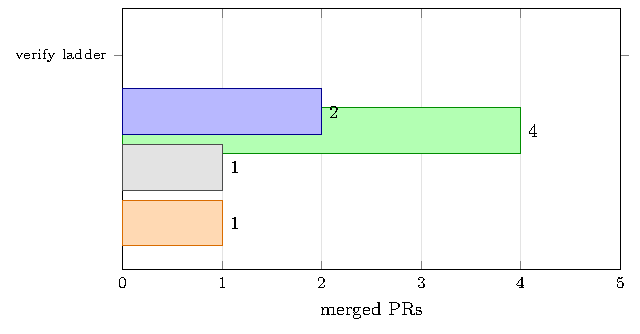
\includegraphics[width=0.80\linewidth]{figures/fig13_pr_roll.pdf}
\caption{The UFO capstone PRs grouped by phase
(\texttt{companion/pr-roll.json}): four verify-ladder PRs (V1--V4), two
pipeline PRs (Phase C: \texttt{spec}, \texttt{verify}), one sibling
reference (CERN), and one monograph PR (this volume). The verify ladder
dominates --- the capstone is verify-native, not implementation-heavy.
Counts are PR records, not line counts (the implementation mass lives in
hexa-lang, @D~d3).}
\label{fig:prroll}
\end{figure}

% -------------------------------------------------------------------------
\subsection{Honest scope --- pointer/manifest, not code}
\label{app:prroll-scope}

The roll's diff-stats are small by design. Per @D~d3, implementation code
lives in the canonical hexa-lang \texttt{stdlib/} home; the UFO-side PRs
are docs/manifests, verify ledgers, and absorption metadata. The proven
content (the Stage-1--3 atoms) was \emph{folded by the sibling domains'
PRs}, not by UFO's --- UFO's reuse is an idempotent atlas skip. The roll
therefore measures the capstone's \emph{integration and verification}
work, not new physics code; that separation is itself part of the honest
record.
